%!TEX TS-program = xelatex

%%%%%%%%%%%%%%%%%%%%%%%%%%%%%%%%%%%%%%%%%%%%%%%%%%%%%%%%%%%%%%%%%%%%%%%%%%%%
% BERT Vision : UC Berkeley MIDS - W266 NLP & Deep Learning
% MIDS Summer 2020, Section 1, Daniel Cer, PhD
% Final : BERT Vision
% Authors : Cristopher Benge (cris.benge@berkeley.edu)
%			William Casey King, PhD (cking@ischool.berkeley.edu)
%			Siduo "Stone" Jiang (siduojiang@ischool.berkeley.edu)
%%%%%%%%%%%%%%%%%%%%%%%%%%%%%%%%%%%%%%%%%%%%%%%%%%%%%%%%%%%%%%%%%%%%%%%%%%%%

%%%%%%%%%%%%%%%%%%%%%%%%%%%%%%%%%%%%%%%%%%%%%%%%%%%%%%%%%%%%%%%%%%%%%%%%%%%%
%%% PACKAGES
%%%%%%%%%%%%%%%%%%%%%%%%%%%%%%%%%%%%%%%%%%%%%%%%%%%%%%%%%%%%%%%%%%%%%%%%%%%%

\documentclass[final,colophon]{caldoc}
\RequirePackage{pdfpages}
\RequirePackage{calstyle}
\addbibresource{references.bib}


%%%%%%%%%%%%%%%%%%%%%%%%%%%%%%%%%%%%%%%%%%%%%%%%%%%%%%%%%%%%%%%%%%%%%%%%%%%%
%%% SETUP
%%%%%%%%%%%%%%%%%%%%%%%%%%%%%%%%%%%%%%%%%%%%%%%%%%%%%%%%%%%%%%%%%%%%%%%%%%%%

\author
{
		\href{https://www.linkedin.com/in/siduojiang/}{Siduo Jiang}, 
		\href{https://jackson.yale.edu/person/casey-king/}{William Casey King}, 
		\href{https://cbenge509.github.io/}{Cristopher Benge}
}
\title{BERT \textcolor{calberkeleyblue}{VISION}}
\subtitle{Improving span annotation and classification task performance using parameter-efficient model architectures trained on BERT's hidden state activations}
\department
{
	Natural Language Processing with Deep Learning (W266)
	\and
	Summer 2020, Section 1, Tuesday 6:30pm PST
}
\faculty{Daniel Cer PhD, Joachim Rahmfeld, Mark Butler, Sid J Reddy PhD, Mike Tamir PhD, Drew Plant, Gurdit Chahal}
\githubrepo{BERTVision}{https://github.com/cbenge509/BERTVision}

\includeonly
{
	chapters/abstract,
	chapters/background,
	chapters/methods,
	chapters/results,
	chapters/bibliography,
	chapters/appendix,
}

\renewcommand\thechapter{\arabic{chapter}}

%%%%%%%%%%%%%%%%%%%%%%%%%%%%%%%%%%%%%%%%%%%%%%%%%%%%%%%%%%%%%%%%%%%%%%%%%%%%
%%% BUILD DOCUMENT
%%%%%%%%%%%%%%%%%%%%%%%%%%%%%%%%%%%%%%%%%%%%%%%%%%%%%%%%%%%%%%%%%%%%%%%%%%%%

\begin{document}

%    \frontmatter

	\caltitle

    \tableofcontents
%	\listoffigures
%	\listoftables
	
	\setcounter{chapter}{1}\setcounter{section}{0}
	\begin{abstract}
Abstract goes here.  This is some filler text to give you an idea
of how the wrapping and margins work for the paper abstract.  You are free
to change whatever text you like here, so long as Daniel Cer thinks its cool.
That's what Casey would say, anyways - we want to make sure Dan is, like, so super comfortable and everything.
\end{abstract}

	\setcounter{chapter}{2}\setcounter{section}{0}
	\section{Background}

Background section

	\setcounter{chapter}{3}\setcounter{section}{0}
	\section{Methods}
\label{sec:methods}

This section introduces our baseline BERT model, and custom models trained on BERT embeddings. We also describe how we use the SQuAD 2.0 question-answering dataset for both span annotation and classification.

\subsection{Modeling approach}

Our custom models use the BERT activations from each encoder layer as input data. For a single SQuAD 2.0 example, our data point has a shape of (X,1024, 25), where $X=386$ for span annotation, and 1 for classification (see appendix [\ref{sec:appendix}] for details). We term this representation of the data as \textit{“embeddings.”}

\subsection{Learned and average pooling}

We implemented the pooling method described in \cite{tenney-etal-2019-bert}, which contracts the last dimension from 25 to 1 through a learned linear combination of each layer. We call this approach learned pooling (LP). We also evaluate the pooling approach reported in \cite{ma2019universal}, average pooling (AP), where each encoder layer is given equal weights. 

\subsection{Adapter compression}

We use the term “compression” to refer to methods that reduce the 1024 dimension of the BERT embeddings. The method proposed in \cite{DBLP:journals/corr/abs-1902-00751} is termed \textit{“adapter”}, which is an auto-encoder type architecture wherein the embeddings are first projected into a lower dimension using a fully-connected layer. For our purposes, the adapter serves as a bridge between BERT embeddings and downstream layers. The architecture in Houlsby et. al. can only handle 3D tensors (including batch), because each adapter handles data from a single transformer layer. Since we work with the activations from multiple layers at once, we need to be able to handle 4D tensors. To do this, our adapter implementation can treat each transformer layer as independent, learning separate compression weights for each layer. Alternatively, we can also employ weight-sharing, so that the compression for each encoder layer follows the same set of transformations.

\subsection{Custom CNN's}

We also implemented various novel CNN architectures, as well as modified existing models such as Inception and Xception \citep{DBLP:journals/corr/SzegedyLJSRAEVR14, DBLP:journals/corr/Chollet16a}. For span annotation, the key is that the CNN models must preserve the text length dimension of 386 (see appendix [\ref{sec:appendix}] for rationale). To view a notebook of all models we tried and their summaries, see: \href{https://github.com/cbenge509/BERTVision}{BERT Vision GitHub repo}.

\subsection{Fine-tuning BERT}

For all experiments, we use the $BERT_{LARGE}$ uncased implementation from \href{https://huggingface.co/}{Hugging Face}. To establish a baseline for our QA tasks, we fine-tuned BERT for 6 epochs with a setup similar to that described in \cite{Devlin2019}. For QA span annotation, questions that do not have answers have the start and end span positions assigned at the CLS token (position 0). We used the Adam optimizer with an initial learning rate of 1e-5. Due to hardware constraints, we use batch size of 8 rather than 48. At inference time, the most likely complete span is predicted based on the maximum softmax probability of the start- and end-span position. The setup is identical in classification, except that we used the pooled CLS token rather than the sequence outputs.
%\begin{equation} \label{eq1}
%Y_{\left(S,E\right)} = \left(\underset{start}{\arg\max} ,\; \underset{end}{\arg\max}\right)
%\end{equation}

\subsection{Ensembling} 

We evaluated multiple ensemble approaches for span annotation. The most successful method presented in this paper takes the element-wise max of the softmax probabilities output by each model. This occurs independently for the start-span position and end-span position. The most likely complete span is then determined by the product of the generated start \& end span vectors.
\begin{equation} \label{eq2}
\begin{aligned}
\text{Let Z be all model softmax probabilities}, \\
K = 386,\;\text{and}\;N = len(Z) \\
\arg\max\left(\prod_{i=1}^{K}{\prod_{j=1}^{N}{Z_{j,i}}}\right)
\end{aligned}
\end{equation}

\subsection{Data processing and evaluation}

We use SQuAD 2.0 for our QA dataset. Standard Exact Match (EM) and F1-score (F1) are used for evaluation as outlined in \cite{DBLP:journals/corr/abs-1806-03822}. For classification, EM is equivalent to accuracy as we are predicting a single binary outcome. For our BERT models, we restrict the maximum token length to 386 (See appendix [\ref{sec:appendix}] for rationale). Question-context pairs that exceed this maximum sequence are split into multiple segments (as many as needed) with an overlap between each segment of 128 tokens. For the splits that do not contain the answer, the labels for that split are set to “no answer”. At inference time, we take the argmax of the span probabilities predicted by each split as the final prediction for the example.
%\begin{equation} \label{eq3}
%EM = \begin{cases} \frac{1}{N}\sum_{i=1}^{N}{\left(\bar{s_i} = s_i,\;\bar{e_i} = e_i\right)} &\mbox{\small if QA} \\
%	\frac{1}{N}\sum_{i=1}^{N}{\left(\bar{s_i} = s_i\right)} &\mbox{\small else}
%	\end{cases} 
%\end{equation}

	\setcounter{chapter}{4}\setcounter{section}{0}
	\section{Results}

\subsection{BERT Fine-Tuning Partial \& Full Epochs}

In order to establish a baseline performance, we fine-tuned BERT for up to 6 epochs with results shown in Figure [\ref{fig:QnABertPerformance}]. We measure performance for every 10th of a fractional epoch between 0 and 1 epochs, as well as full epochs up to 6. We observed that performanced peaked at 2 epochs, achieving an Exact Match (EM) of 0.747, and an F1 score of 0.792. Between 0 and 1 epochs, performance consistently increased both in terms of EM and F1. For comparison with other published works, see Appendix. \\

In order to select where to extract our hidden state activations, we chose 2 time points to balance training time and model performance. The first is a full training epoch. On our GPU, fine-tuning for 1 epoch is expensive and takes around 5 hours, but performance is already relatively decent compared to peak performance at 2 epochs. This time point gives us high quality embeddings for model development. The second time point is 3/10 of an epoch, which takes about 1.5hr to fine-tune. While cheaper, at this time point, the model has yet to achieve the large jump in performance observed between 3/10 and 4/10 of an epoch. This provides us an opportunity for improvement using our models. 

\begin{figure}[ht]
	\centering
	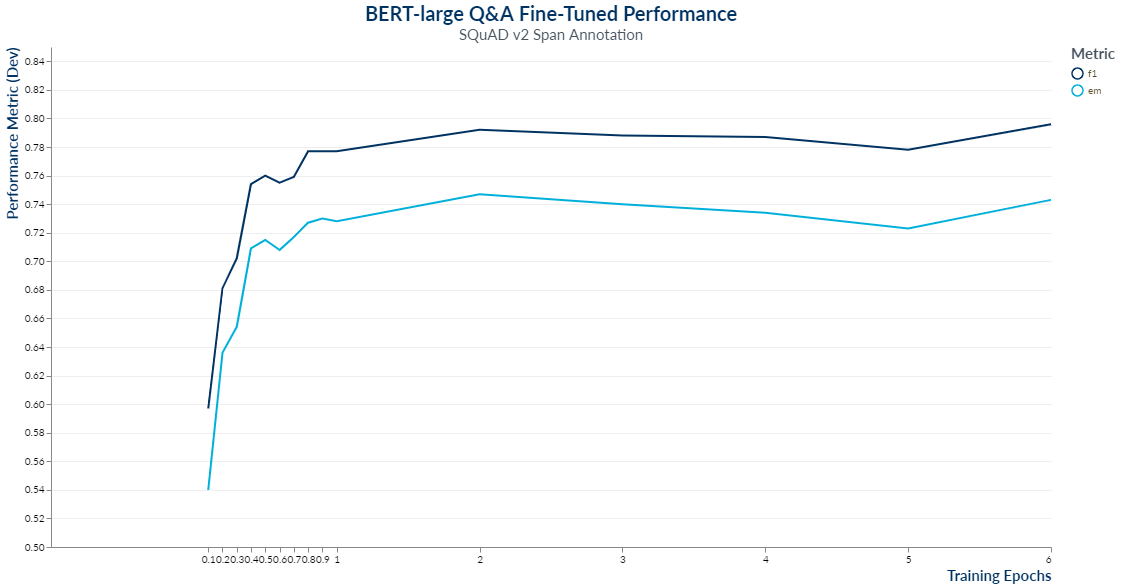
\includegraphics[width=75mm]{images/QnA_BERT_Training_Performance_plot.png}
	\caption{\label{fig:QnABertPerformance}QnA Performance, BERT SQuAD 2.0}
\end{figure}

\subsection{Models trained at 3/10 epoch BERT embeddings}

Using the embeddings at 3/10 of epoch, we explored over 20 parameter-efficient models using a combination of CNNs, pooling and compression techniques. Table [?] shows the performance of our most promising models, and results of all models are in the Appendix. \\

First, we compared two pooling strategies. Our LP (learned pooling) model is identical to the pooling model outlined in Tenney et. al. [?], where weights for combining each encoder layer is learned. The AP (average pooling) model proposed by Ma et. al. [?] on the other hand weights each encoder layer equally. We found that an LP model achieved similar performance as BERT itself, while average pooling significantly decreased performance. An analysis of the learned weights suggests that a non-uniform distribution of pooling weights is optimal, with the distribution slightly favoring later layers of BERT compared to earlier layers (see Appendix). \\

Next, we evaluated the possibility of using adapters modified from Houlsby et. al (see Methods). We found that our modified adapters of all flavors improved model performance compared to baseline BERT. Our best model uses an adapter of size of 386 with weight sharing enabled for each encoder layer, achieving an EM of 0.699 and F1 of 0.740. A skip connection between the final encoder layer and our model’s penultimate hidden layer is also included (see Figure [?]). Without weight-sharing, the number of parameters increases by about 24x, and model performance slightly decreases. While Houlsby et. al. found that an adapter size of 64 provides the best F1 score when used in between transformer blocks, for our purposes, a size of 64 performed worse with or without weight-sharing. Our best adapter model significantly beats BERT fine-tuned to the same level of 3/10 of an epoch by about 4 percentage points in both EM and F1, although we failed to reach performance at 1 full epoch. \\

While we extensively explored stacking pooling with adapters and CNNs, we did not find a model which performed better than our best adapter model. For example, Table [\ref{tbl:3_10_Models}] shows a model where we stacked learned pooling with our best adapter model and abbreviated Xception network. The number of parameters increased by 16x, but performance was no better than pooling alone.

\begin{table}[ht]
	\centering
	\small
	\begin{tabular}{L{3.5cm} C{0.6cm} C{0.6cm} C{0.6cm} C{0.6cm}}
		\hline
		\textbf{Model} (\% params of $BERT_{LARGE}$)       & \textbf{EM $\frac{3}{10}e$} & \textbf{F1 $\frac{3}{10}e$} & \textbf{EM $1e$} & \textbf{F1 $1e$}\Tstrut \\
		\hline
		BERT $\frac{3}{10}e\;\left(100\%\right)$           & $0.654$ & $0.702$ & $0.728$ & $0.777$\Tstrut\Bstrut  \\
		BERT $1e\;\left(100\%\right)$ 					   & $0.670$ & $0.712$ & $0.728$ & $0.777$\Tstrut\Bstrut  \\
		learned pooling $\left(0.001\%\right)$             & $0.660$ & $0.703$ & $0.725$ & $0.759$\Tstrut\Bstrut  \\
		average pooling $\left(0.001\%\right)$             & $0.657$ & $0.700$ & $0.736$ & $0.741$\Tstrut\Bstrut  \\
		\hline\hline
		adapter shared 386 skip $\left(0.124\%\right)$     & \boldmath$0.699$ & \boldmath$0.740$ & \boldmath$0.745$ & \boldmath$0.791$\Tstrut\Bstrut  \\
		\hline\hline
		adapter independent 386 $\left(2.957\%\right)$     & $0.676$ & $0.723$ & $0.730$ & $0.778$\Tstrut\Bstrut  \\
		adapter shared 64 $\left(0.021\%\right)$           & $0.680$ & $0.732$ & $0.722$ & $0.761$\Tstrut\Bstrut  \\
		adapter independent 64$\left(0.491\%\right)$         & $0.684$ & $0.716$ & $0.736$ & $0.782$\Tstrut\Bstrut  \\
		pooling adapter 386 \& xception $\left(1.970\%\right)$         & $0.668$ & $0.711$ & $0.699$ & $0.751$\Tstrut\Bstrut  \\
		\hline
	\end{tabular}
	\caption{\label{tbl:3_10_Models}Models at $\frac{3}{10}$ epochs but evaluated at 1 epoch}
\end{table}

\subsection{Best Models on top at 1 epoch}

Using the embeddings at 1 epoch of fine-tuning, we trained the same set of 20 models as at 3/10 of an epoch of fine-tuning (see the Appendix for a full set of results). In most cases, we found that our models outperformed BERT at 1 epoch of fine-tuning. One exception is our adapter 386 model with independent weights, which suffered about 1 percentage point drop. Table [\ref{dev_set_performance}] shows that adapter models of size 64, with or without weight-sharing, both beat BERT, but the best model found is almost identical to that found at 3/10 of an epoch utilizing an adapter size of 386. The only exception that a skip connection is not needed in this case. This model’s performance is also competitive with maximum performance achieved with BERT fine-tuning, with a slightly improved EM (0.749 vs 0.747) and a slightly decreased F1 (0.790 vs 0.792). This result shows that we are able to reduce BERT fine-tuning by 1 epoch and still achieve similar performance with a model of only about 0.124\% of the number of BERT parameters. 

\begin{table}[ht]
	\centering
	\small
	\begin{tabular}{L{2.8cm} L{1.8cm} C{0.6cm} C{0.6cm}}
		\hline
		\textbf{Model} & \textbf{\% params of} $BERT_{LARGE}$ & \textbf{EM} & \textbf{F1}\Tstrut \\
		\hline
		BERT $1e$ & 100\% 						 & $0.728$ & $0.777$ \\
		BERT $2e$ (\textit{best}) & 100\%		 & $0.747$ & $0.792$ \\
		adapter shared 386 & 0.124\% 			 & $0.749$ & $0.790$ \\
		\hline\hline
		adapter independent 386 & 2.957\% 		 & \boldmath$0.716$ & \boldmath$0.767$ \\
		\hline\hline
		adapter shared 64 & 0.021\% 			 & $0.739$ & $0.785$ \\
		adapter independent 64 & 0.491\% 		 & $0.736$ & $0.784$ \\
		tenney adapter 386 \& xception & 1.970\% & $0.741$ & $0.786$ \\
		\hline
	\end{tabular}
	\caption{\label{tbl:dev_set_performance}Dev set performance}
\end{table}

\subsection{Performance of models trained at 3/10 epoch on higher quality embeddings}

We wanted to better understand why models trained on embeddings derived at 1 epoch of fine-tuning performed better than models trained on embeddings derived at 3/10 of an epoch. In order to do this, we took all of our models trained on the 3/10 embeddings, and evaluated their performance on the dev set with embeddings derived at 1 epoch. To our surprise, all models experienced a significant jump in performance compared to evaluation at embeddings derived at 3/10 of an epoch. Figure [?] shows a comparison of these results on our top models, and Appendix S[?] contains data for all models.  \\

For example, our best model trained at 3/10 of an epoch achieved a performance of 0.745 EM and 0.791 F1 when evaluated on embeddings from 1 epoch. This is a significant boost compared to evaluating the exact same model on embeddings derived from 3/10 of an epoch (0.699 EM and 0.740EM). This model performs similarly to our best model trained on 1 epoch embeddings, and by a transitive relation, also performs similarly to maximum BERT performance at 2 epochs. We consider this a significant achievement for a model that has only seen data from 3/10 of an epoch of fine-tuning. \\

Our result suggests that models trained at 3/10 of an epoch are learning transformations that are transferable even as BERT is further fine-tuned. This implies that BERT is maintaining some level of constancy in the structure of its internal representations. Practically, this means that our models can be trained in parallel with BERT fine-tuning. As BERT learns better internal representations of the data, models trained on earlier representations can leverage this improvement and achieve better performance on the task on hand. \\

\subsection{Training with less data}

The previous sections show that our models perform well compared to BERT when trained on the full dataset. However, since supervised data can be difficult to obtain for certain tasks, we wanted to explore whether our models can perform well with significantly less data. In addition in our case, since embeddings can be expensive to calculate and store, reducing training data also helps with our data management issue (see Methods). To answer this question, we trained our best models (for both 3/10 epoch and 1 epoch embeddings) on varying amounts of data, ranging from 0\% to 100\% of the dataset at step sizes of 10\%. All models were trained for 1 epoch, the same as using the full dataset. Here, 0\% represents randomized weights with no training. For the model at 3/10 of an epoch, we measured its dev set performance on both the 3/10 epoch embeddings and 1 epoch embeddings.  \\

Figure [\ref{fig:1_epoch_embeddings__adapter_386_with_skip}] shows the results. In all cases, we rapidly approach strong performance early on, beating BERT at around 30\% of the data. Even at 10\% of the data, we are only about 3 percentage points in terms of EM, and 2 from F1, from maximum peak performance. This shows that we can in fact achieve strong performance even when using training less. 

\begin{figure}[ht]
	\centering
	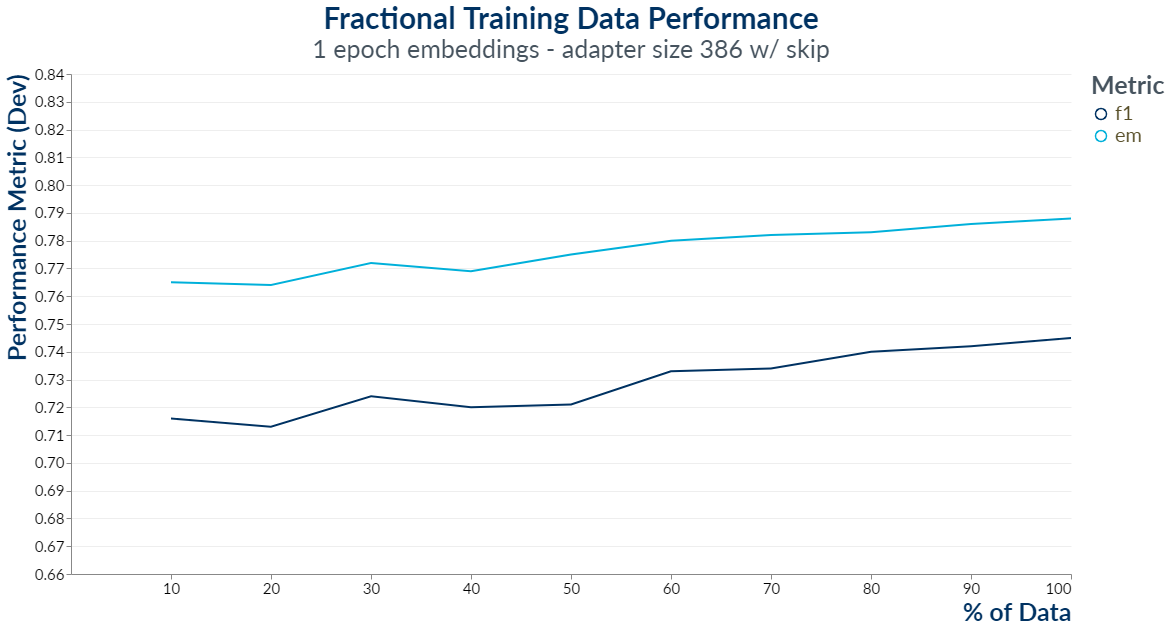
\includegraphics[width=75mm]{images/1_Epoch_Embeddings__Adapter_386_with_Skip.png}
	\caption{\label{fig:1_epoch_embeddings__adapter_386_with_skip}1 epoch embeddings - adapter 386 w/ skip}
\end{figure}

\begin{table}[ht]
	\centering
	\small
	\begin{tabular}{L{0.8cm} C{0.90cm} C{0.90cm} C{1.5cm} C{1.5cm}}
		\hline\Bstrut
		\textbf{\% data} & \textbf{EM} & \textbf{F1} & \textbf{EM \boldmath$1e$ embeddings} & \textbf{F1 \boldmath$1e$ embeddings}  \\
		\hline\Tstrut\Bstrut
		10\%  & $0.633$ & $0.692$ & $0.712$ & $0.768$ \\[.1cm]
		20\%  & $0.633$ & $0.690$ & $0.714$ & $0.767$ \\[.1cm]
		30\%  & $0.660$ & $0.711$ & $0.735$ & $0.782$ \\[.1cm]
		40\%  & $0.663$ & $0.695$ & $0.737$ & $0.775$ \\[.1cm]
		50\%  & $0.673$ & $0.712$ & $0.741$ & $0.783$ \\[.1cm]
		60\%  & $0.681$ & $0.719$ & $0.733$ & $0.772$ \\[.1cm]
		70\%  & $0.683$ & $0.729$ & $0.731$ & $0.779$ \\[.1cm]
		80\%  & $0.686$ & $0.724$ & $0.741$ & \boldmath$0.785$ \\[.1cm]
		90\%  & $0.687$ & $0.734$ & $0.733$ & $0.783$ \\[.1cm]
		100\% & \boldmath$0.689$ & \boldmath$0.733$ & \boldmath$0.736$ & $0.783$ \\[.1cm]
		\hline
	\end{tabular}
	\caption{\label{tbl:3_10_embeddings__adpater_386}$\frac{3}{10}$ Epochs embeddings - adapter 386}
\end{table}




	%----------------------------------------------------------------------------------------
	%	BIBLIOGRAPHY
	%----------------------------------------------------------------------------------------

	\setcounter{chapter}{5}\setcounter{section}{0}
	% =====================================================================================================
%
%  BIBLIOGRAPHY
%
% =====================================================================================================
\begingroup
\renewcommand{\cleardoublepage}{}
\renewcommand{\clearpage}{}
\chapter*{Bibliography}\label{chap:biblio}
\addcontentsline{toc}{chapter}{Bibliography}
\renewcommand{\chapter}[2]{}%q

\nocite{*}
\printbibliography

\endgroup


	\setcounter{chapter}{6}\setcounter{section}{0}
	\appendix

\section{Appendices}
\label{sec:appendix}
\small

\subsection{BERT fine-tuning figures}
\label{apdx:BERT_fine_tuning_span_annotation_sec}

BERT$_{large}$ was fine-tuned for both span annotation and classification tasks; below are tables and blots indicating the performance for each task.

\begin{figure}[h]
	\centering
	\begin{subfigure}{0.95\textwidth}%
		\centering
		\includegraphics[width=\linewidth]{images/classification/BERT_Large_Training.png}%
		\caption{BERT$_{large}$ fine-tuning table : classification}
	\end{subfigure}%

	\vspace*{8pt}%
	
	\begin{subfigure}{0.96\textwidth}%
		\centering
		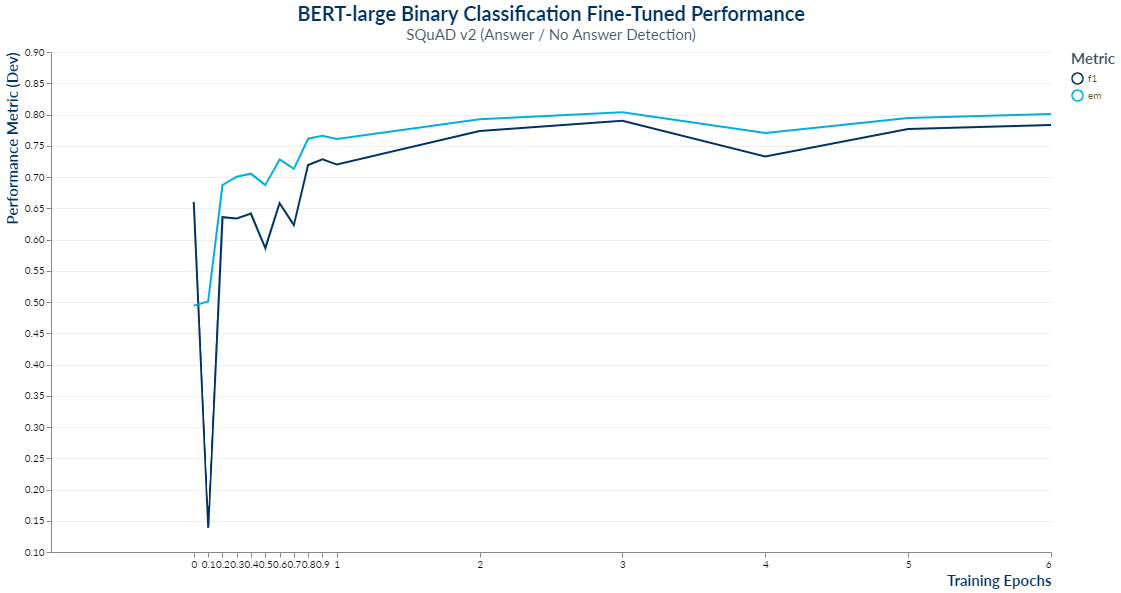
\includegraphics[width=\linewidth]{images/BinaryClassification_BERT_Training_Performance_plot.png}%
		\caption{BERT$_{large}$ fine-tuning plot : classification}
	\end{subfigure}%
	\caption{\label{apdx:BERT_fine_tuning_classification}BERT$_{large}$ fine-tuning for classification}
\end{figure}%

\begin{figure}[!h]
	\centering
	\begin{subfigure}{0.95\textwidth}%
		\centering
		\includegraphics[width=\linewidth]{images/span/BERT_Large_Training.png}%
		\caption{BERT$_{large}$ fine-tuning table : span annotation}
	\end{subfigure}%
	
	\vspace*{8pt}%

	\begin{subfigure}{0.96\textwidth}%
		\centering
		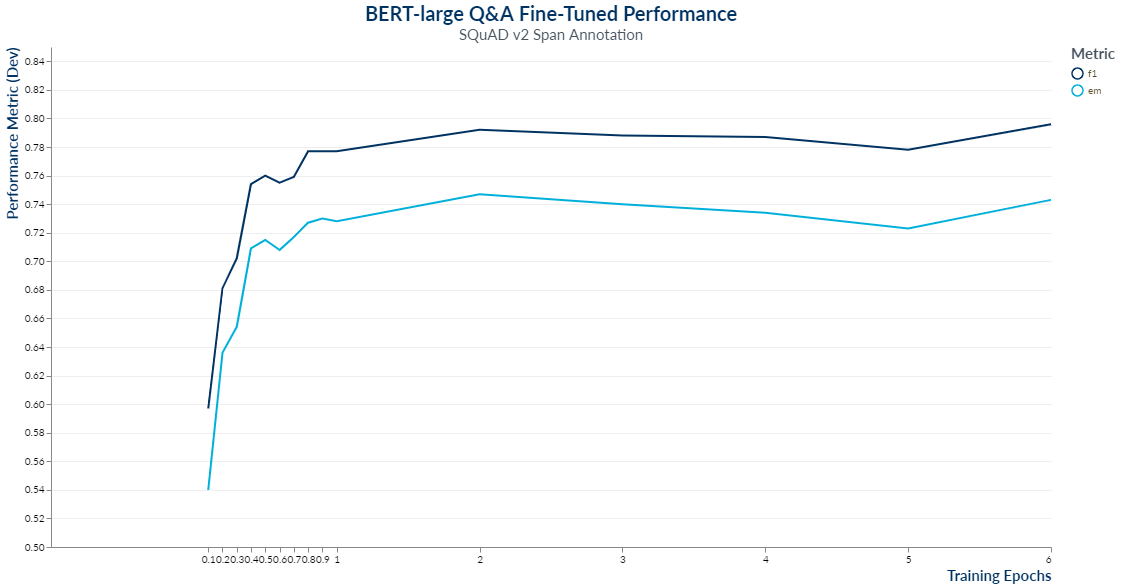
\includegraphics[width=\linewidth]{images/QnA_BERT_Training_Performance_plot.png}%
		\caption{BERT$_{large}$ fine-tuning plot : span annotation}
	\end{subfigure}%
	\caption{\label{apdx:BERT_fine_tuning_span_annotation}BERT$_{large}$ fine-tuning for span annotation}
\end{figure}

\newpage
\subsection{Table of all model results for span annotation}
\label{apdx:span_annotation_all_results}

Models were trained on embeddings derived from 3/10 of an epoch and 1 full epoch.  Performance on evaluation of the dev set is presented below.

\begin{figure}[h]
	\centering
	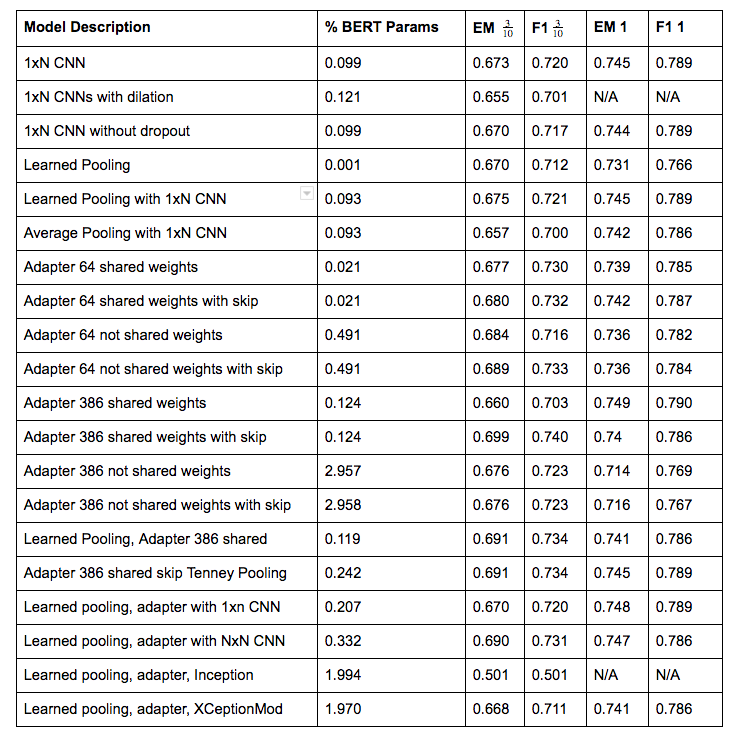
\includegraphics[width=\linewidth]{images/span/Span_Annotation_All_Model_Results.png}%
	\caption{BERT$_{large}$ All model performance : span annotation}
\end{figure}

\subsection{Best model performance for classification task}

The best model evaluated for the classification task was a simple linear model that performed channel contraction using learned weights followed by a simple dense layer connection with no softmax.  As indicated below, this model outperformed BERT$_{large}$ for almost every metric save for F1 on 3 epoch fine-tuned embeddings.

\begin{figure}[h]
	\centering
	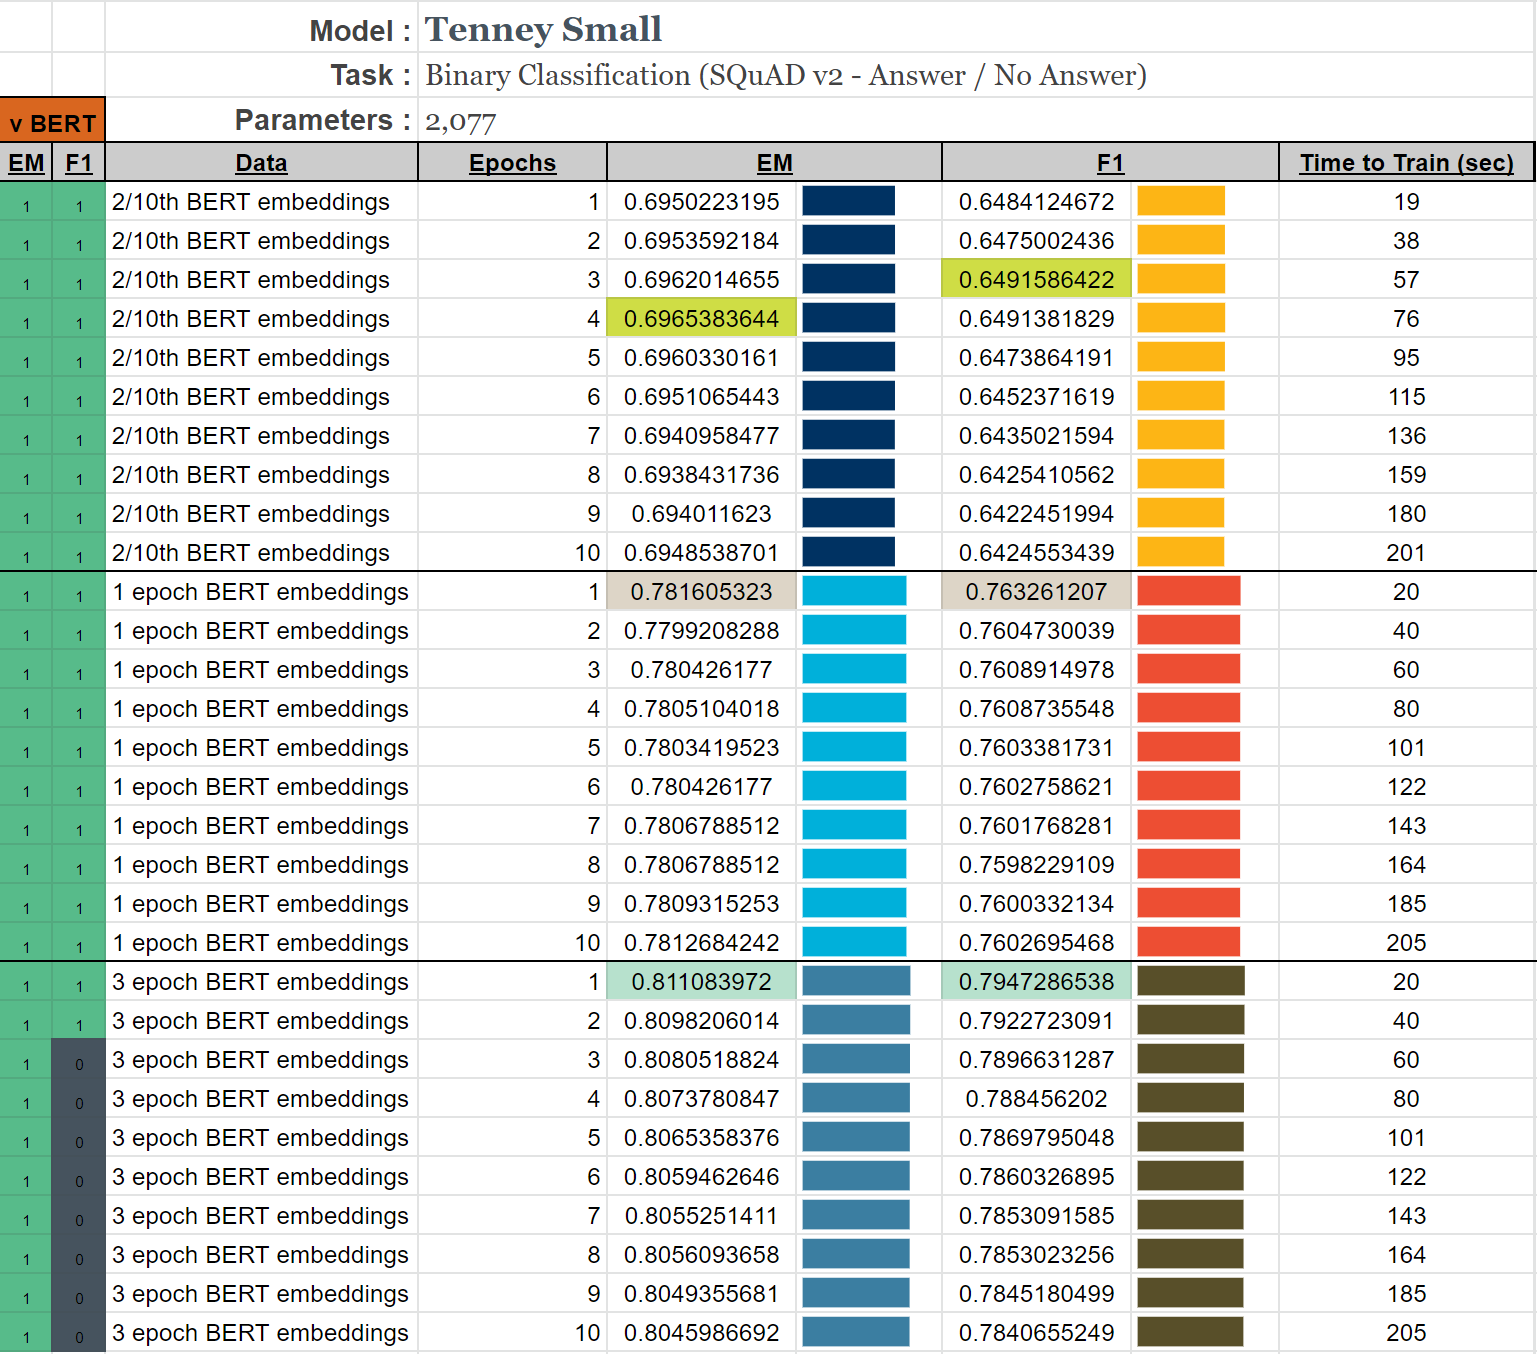
\includegraphics[width=\linewidth]{images/classification/TenneySmall_Training.png}%
	\caption{BERT$_{large}$ Best model performance : classification task}
\end{figure}

\newpage

\begin{figure*}[t]
	\centering
	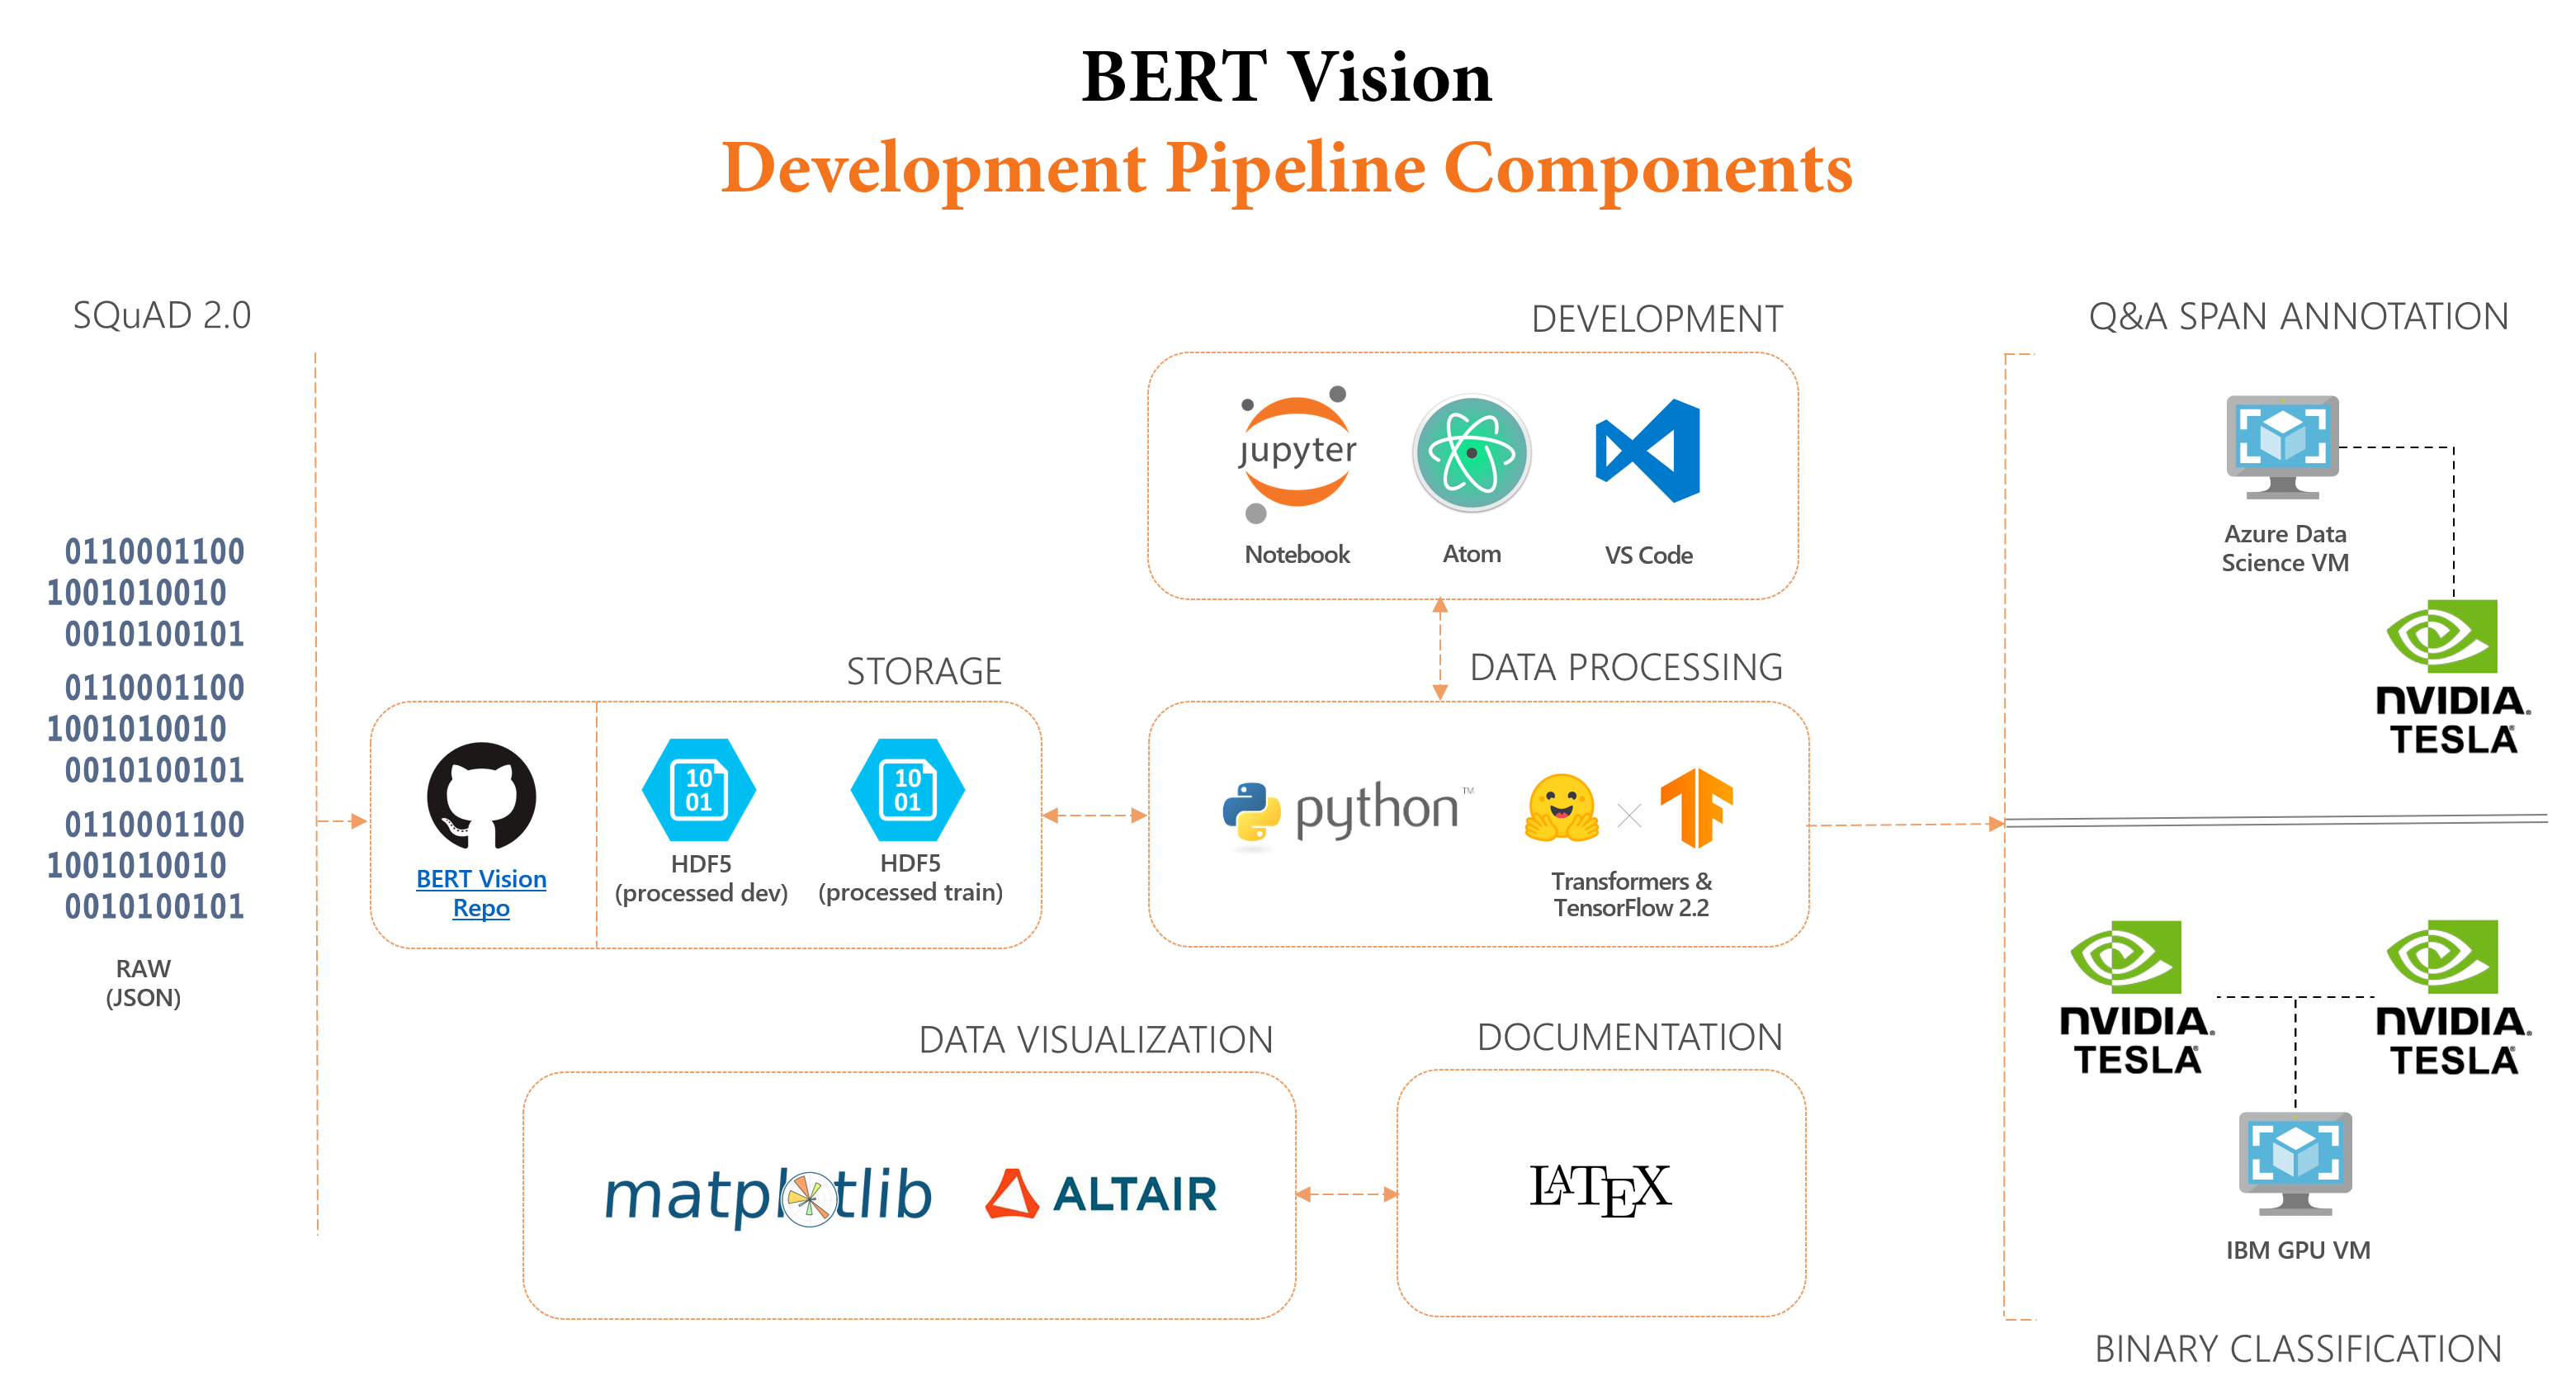
\includegraphics[width=\textwidth]{images/BERTVision_Development_PIpeline.png}%
	\caption{BERTVision development pipeline}
	\label{apdx:bertvision_development_pipeline_graph}
\end{figure*}

\newpage

\subsection{Table of all model results for classification}
\label{apdx:classification_models_trained}

Models were trained on BERT$_{large}$ fine-tuned embeddings derived from 2/10 of an epoch and 1 full epoch. Additionally, the most successful model was trained on 3 epochs fine-tuned embeddings. Performance on evaluation of the dev set is presented below.

\begin{table}[h]
	\centering
	\small
	\begin{tabular}{L{2.9cm}|C{1.5cm} C{0.9cm} C{0.9cm}}
		\toprule
		\textbf{Model} & \textbf{\% Params} & \multicolumn{2}{c}{\textbf{SQuAD2.0}}\\
		& \textbf{BERT}$_{large}$ & \textbf{EM} & \textbf{F1}\\
		\midrule
		adapter pooler tenney 	& 0.119\% & 0.685 & 0.646 \\
		xception abbr 			& 0.079\% & 0.673 & 0.702 \\
		\textbf{xception}		& \textbf{6.181\%} & \textbf{0.707} & \textbf{0.710} \\
		xception abbr cls 		& 0.080\% & 0.672 & 0.564 \\
		adapter pooler avg 		& 0.119\% & 0.691 & 0.624 \\
		tenney small 			& 0.001\% & 0.697 & 0.650 \\
		\bottomrule
	\end{tabular}
	\caption{Models trained on embeddings at $\frac{2}{10}e$}
\end{table}

\begin{table}[h]
	\centering
	\small
	\begin{tabular}{L{2.9cm}|C{1.5cm} C{0.9cm} C{0.9cm}}
		\toprule
		\textbf{Model} & \textbf{\% Params} & \multicolumn{2}{c}{\textbf{SQuAD2.0}}\\
		& \textbf{BERT}$_{large}$ & \textbf{EM} & \textbf{F1}\\
		\midrule
		adapter pooler tenney 	& 0.119\% & 0.781 & 0.765 \\
		\textbf{xception abbr}	& \textbf{0.079\%} & \textbf{0.785} & \textbf{0.782} \\
		xception 				& 6.181\% & 0.783 & 0.766 \\
		xception abbr cls 		& 0.080\% & 0.783 & 0.780 \\
		adapter pooler avg 		& 0.119\% & 0.779 & 0.765 \\
		tenney small 			& 0.001\% & 0.782 & 0.763 \\
		\bottomrule
	\end{tabular}
	\caption{Models trained on embeddings at $1e$}
\end{table}

\begin{table}[h]
	\centering
	\small
	\begin{tabular}{L{2.9cm}|C{1.5cm} C{0.9cm} C{0.9cm}}
		\toprule
		\textbf{Model} & \textbf{\% Params} & \multicolumn{2}{c}{\textbf{SQuAD2.0}}\\
		& \textbf{BERT}$_{large}$ & \textbf{EM} & \textbf{F1}\\
		\midrule
		tenney small & 0.001\% & 0.811 & 0.795 \\
		\bottomrule
	\end{tabular}
	\caption{Models trained on embeddings at $3e$}
\end{table}

\subsection{Data challenges and training time}
\label{apdx:data_challenges}

During training, in order to obtain the internal BERT embeddings for each example (which is the input “data” into our downstream models), we had to either: 1.  Pre-generate the embeddings, or 2. Generate the embeddings for each example on the fly from a frozen BERT model. Due to the size of BERT, we quickly ran out of GPU memory with the second method, so we had to resort to the first. Working with BERT embeddings on the SQuAD 2.0 data set presented a data engineering problem due to the size of the data. Using the 4-byte float representation, the entire dataset with each example having shape (386, 1024, 25) is approximately 5 TB in size, which is far too large to store into memory on our hardware. Instead, this data was written to disk, and a custom Keras data generator used to retrieve this data in batch sizes of 16 for training (in a shuffled random order).

While this method presents no cost to accuracy, the I/O time for loading the data was significant, much longer in most cases than the actual training time for fitting any of our models. For all models, training per epoch was around 5 hours, but we estimate that on average over 95\% of the time is spent on loading data, and only 5\% of the time fitting the model. As a result, in this work, in order to separate out infrastructure issues with model training, as a proxy for training cost, we compare the number of parameters in our model rather than wall clock training time. We also explore the potential to use less embedding data during fitting, and for future work, a faster storage system should be explored in order to advance this work for practical applications. 

We also note that for the classification task, we did not experience any data management issues. Since we only use the CLS token for classification rather than the entire sequence length of 386, the full embeddings of all examples were a little over 13GB, which easily fit into CPU memory. Training for each epoch for on the order of minutes rather than hours.

\subsection{Model training strategy}
\label{apdx:model_training_strategy}

We train all of these models for a single epoch for three reasons: 1. Performance was already desirable at a single epoch. 2. Further training typically did not help performance further, 3. Due to our data management issue, loading the data usually takes more than 95\% of the training time, which makes it difficult to train for extended numbers of epochs (See [\ref{apdx:data_challenges}]). 

\subsection{Explanation on the shape of input embeddings data}
\label{apdx:explanation_of_input_embeddings_shape}

For span annotation, for a single SQuAD 2.0 example, the data point has a shape of (386,1024,25). Here, 386 represents the text length dimension, and 1024 the BERT embedding dimension for each encoder layer. The 25 comes from the stacking of the contextual wordpiece \cite{DBLP:journals/corr/WuSCLNMKCGMKSJL16} text embeddings, the 23 hidden state activations, and the final sequence outputs (24th layer) for BERT. 

For classification, an example has input shape (1,1024, 26). Here, 1 represents the lone CLS token, 1024 the BERT embedding dimension. The 26 comes from the stacking of the contextual wordpiece text embeddings, 23 hidden state activations, the final CLS token for the output encoder layer (24th layer), and the pooled CLS token from the final pooler layer.

\subsection{Explanation on max sequence length input into BERT}
\label{apdx:explanation_max_sequence_length}

BERT$_{large}$ has a maximum input sequence length of 512. While we could have truncated our question-context pairs at this length, we found that a large majority of examples were much shorter than this length. The average length of the input is about 171 tokens long. The length we chose was 386, which is between 98-99th percentile. As a result, without much loss, we can significantly save on the number of mostly meaningless “[PAD]” tokens we needed to store, especially for full 25-layers of BERT embeddings.

\subsection{CNN models preserving max sequence length}
\label{apdx:cnn_models_preserving_seq_length}

Our CNN models were all designed to preserve the sequence length of the input question-context pair. This was achieved with 1xN convolutions so that these filters only compress along the 1024 dimension, or with NxN convolutions with padding along the sequence token dimension. In the case of 1xN convolutions, this is similar to a unigram model that treats each token separately. The NxN convolutions were n-gram models, ranging from 1 - 7 (depending on the size of N). The reason we did this is because we also tried convolution blocks from Inception [1] that gradually shrinks the 386 dimension; however, this model failed to learn to even fit the training data. As a result, we believe that for span annotation, since the data starts with a 386 dimension representing token position, and ends by predicting a probability for each position, we need this sentence length dimension throughout the entire model. A traditional computer vision CNN model such as Inception shrinks the image along this dimension, which destroys the structure necessary for span detection. Shrinking the text length and later expanding it again loses information, resulting in a failure to fit the data.

\subsection{Comparison of our BERT performance with Devlin}
\label{apdx:comparison_with_devlin}

For our fine-tuning procedure, we observed that performance peaked at 2 epochs, achieving an Exact Match (EM) of 0.747, and an F1 score of 0.792. This is slightly worse than that reported by \cite{Devlin2019} at an EM of 78.7 and F1 of 81.9. We hypothesize that these difference might arise due to our training batch size, random initializations, and the fact we do not favor the null answer by a "$\theta$" threshold, where "$\theta$" was optimized based on dev set performance (see Section 4.3 in Devlin). We use purely the softmax probabilities output by the model without favoring no answer by an optimized threshold based on the dev set itself.

\subsection{Where to exact embeddings}
\label{apdx:where_to_extract_embeddings}

We wished to extract embeddings at two stages in the training process: 1. Early-on so that BERT fine-tuning is cheap, and the embeddings are amenable to use as data for modeling, 2. At a slightly later stage before convergence so that our models have a chance to achieve or outcompete the best performing BERT model. 

For span detection, our learning curve for full-epoch BERT fine-tuning shows that 1 epoch is relatively decent compared to peak performance at 2 epochs, which gives us a chance to outperform our best observed BERT performance (goal 2). At the same time, fine-tuning for a full epoch on all of SQuAD 2.0 takes around 5 hours, which is already very expensive. To this end, we explored BERT performance every 1/10 of a fractional epoch between 0 and 1. We see that both EM and F1 are increasing steadily in our single run, with a large jump between fractional epochs 3 and 4. In addition to 1 epoch, we extracted embeddings at 3/10 of an epoch immediately before this jump, which took approximately 1.5 hours of fine-tuning. We believe this is a decent spot because such partial fine-tuning is relatively cheap, and performance has yet to jump, giving us an opportunity to improve performance using our models (goal 1).

For classification, looking at our learning curve for full-epoch fine-tuning, 1 epoch is yet again a clear candidate for extracting the embeddings (goal 2). Performance is already relatively decent compared to peak performance at 3 epochs, but takes $\frac{1}{3}$ time and compute resources to train. For goal 1, we extracted embeddings at 2/10 of a fractional epoch between 0 and 1. We see a clear jump in performance between 1/10 of a fractional epoch and 2/10, a jump we do not observe again until 8/10. Therefore, from the dev set perspective, 2/10 is a high value fractional epoch, whether 3/10 - 7/10 does not add much to the performance of the model.

\subsection{Need to fine-tune}
\label{adpx:need_to_fine_tune}

Using a variety of parameter-efficient CNNs and dense architectures, we found such models were unable to fit BERT hidden state activations without fine-tuning to our specific QA task SQuAD 2.0. This discovery is consistent with the observations made in \cite{ma2019universal}, where the authors found that fine-tuned BERT on either SNLI and in-domain text corpus consistently outperformed pre-trained BERT without fine-tuning by a large margin for various tasks, including QA (although not on SQuAD). As a result, we decided mild amounts of fine-tuning was necessary in order to generate usable embeddings.

\subsection{Training hardware and development pipeline}
\label{apdx:training_hardware}

All span annotation training and inferencing was performed on a Microsoft Azure data science virtual machine with 112GiB onboard ram and a single NVIDIA Tesla TITAN series V100 Tensor Core GPU capable of ~7 TFLOPS double-precision and tensor performance of ~112 TFLOPS and possessed 16 GiB onboard RAM.  All binary classification training and experimentation was performed on an IBM virtual machine equipped with two NVIDIA Tesla TITAN series V100 Tensor Core GPU's (see [\ref{apdx:bertvision_development_pipeline_graph}]).

\begin{figure*}[t]
	\centering
	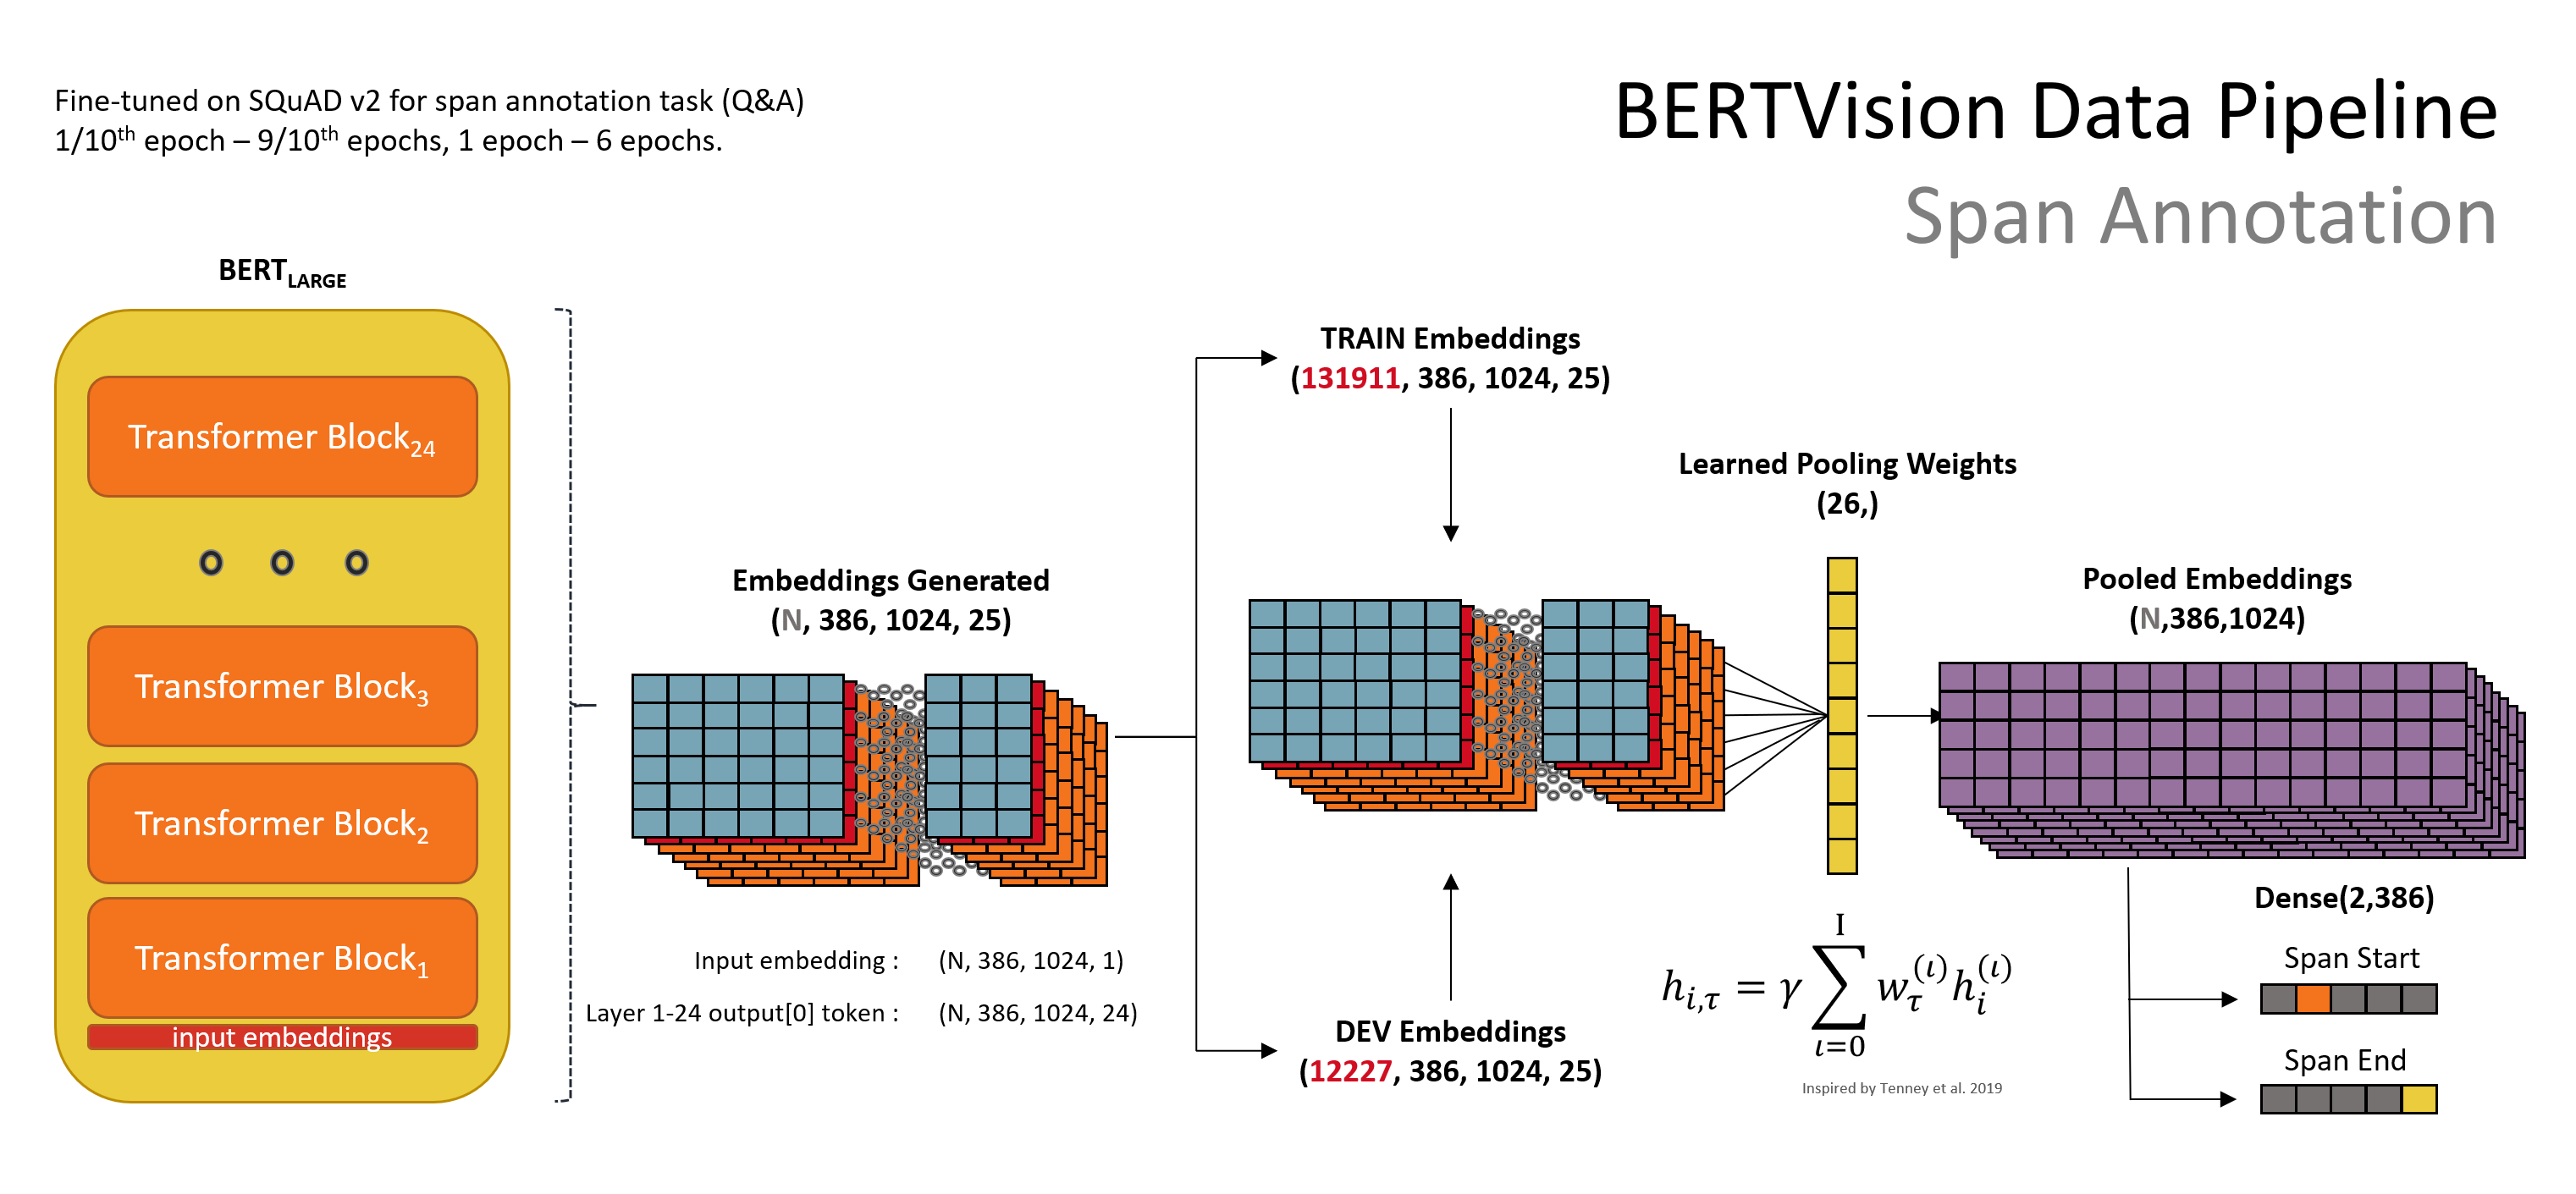
\includegraphics[width=\textwidth]{images/Data_Pipeline_Span_Annotation.png}%
	\caption{BERTVision span annotation data pipeline}
	\label{apdx:bertvision_span_annotation_data_pipeline_graph}
\end{figure*}

\begin{figure*}[!h]
	\centering
	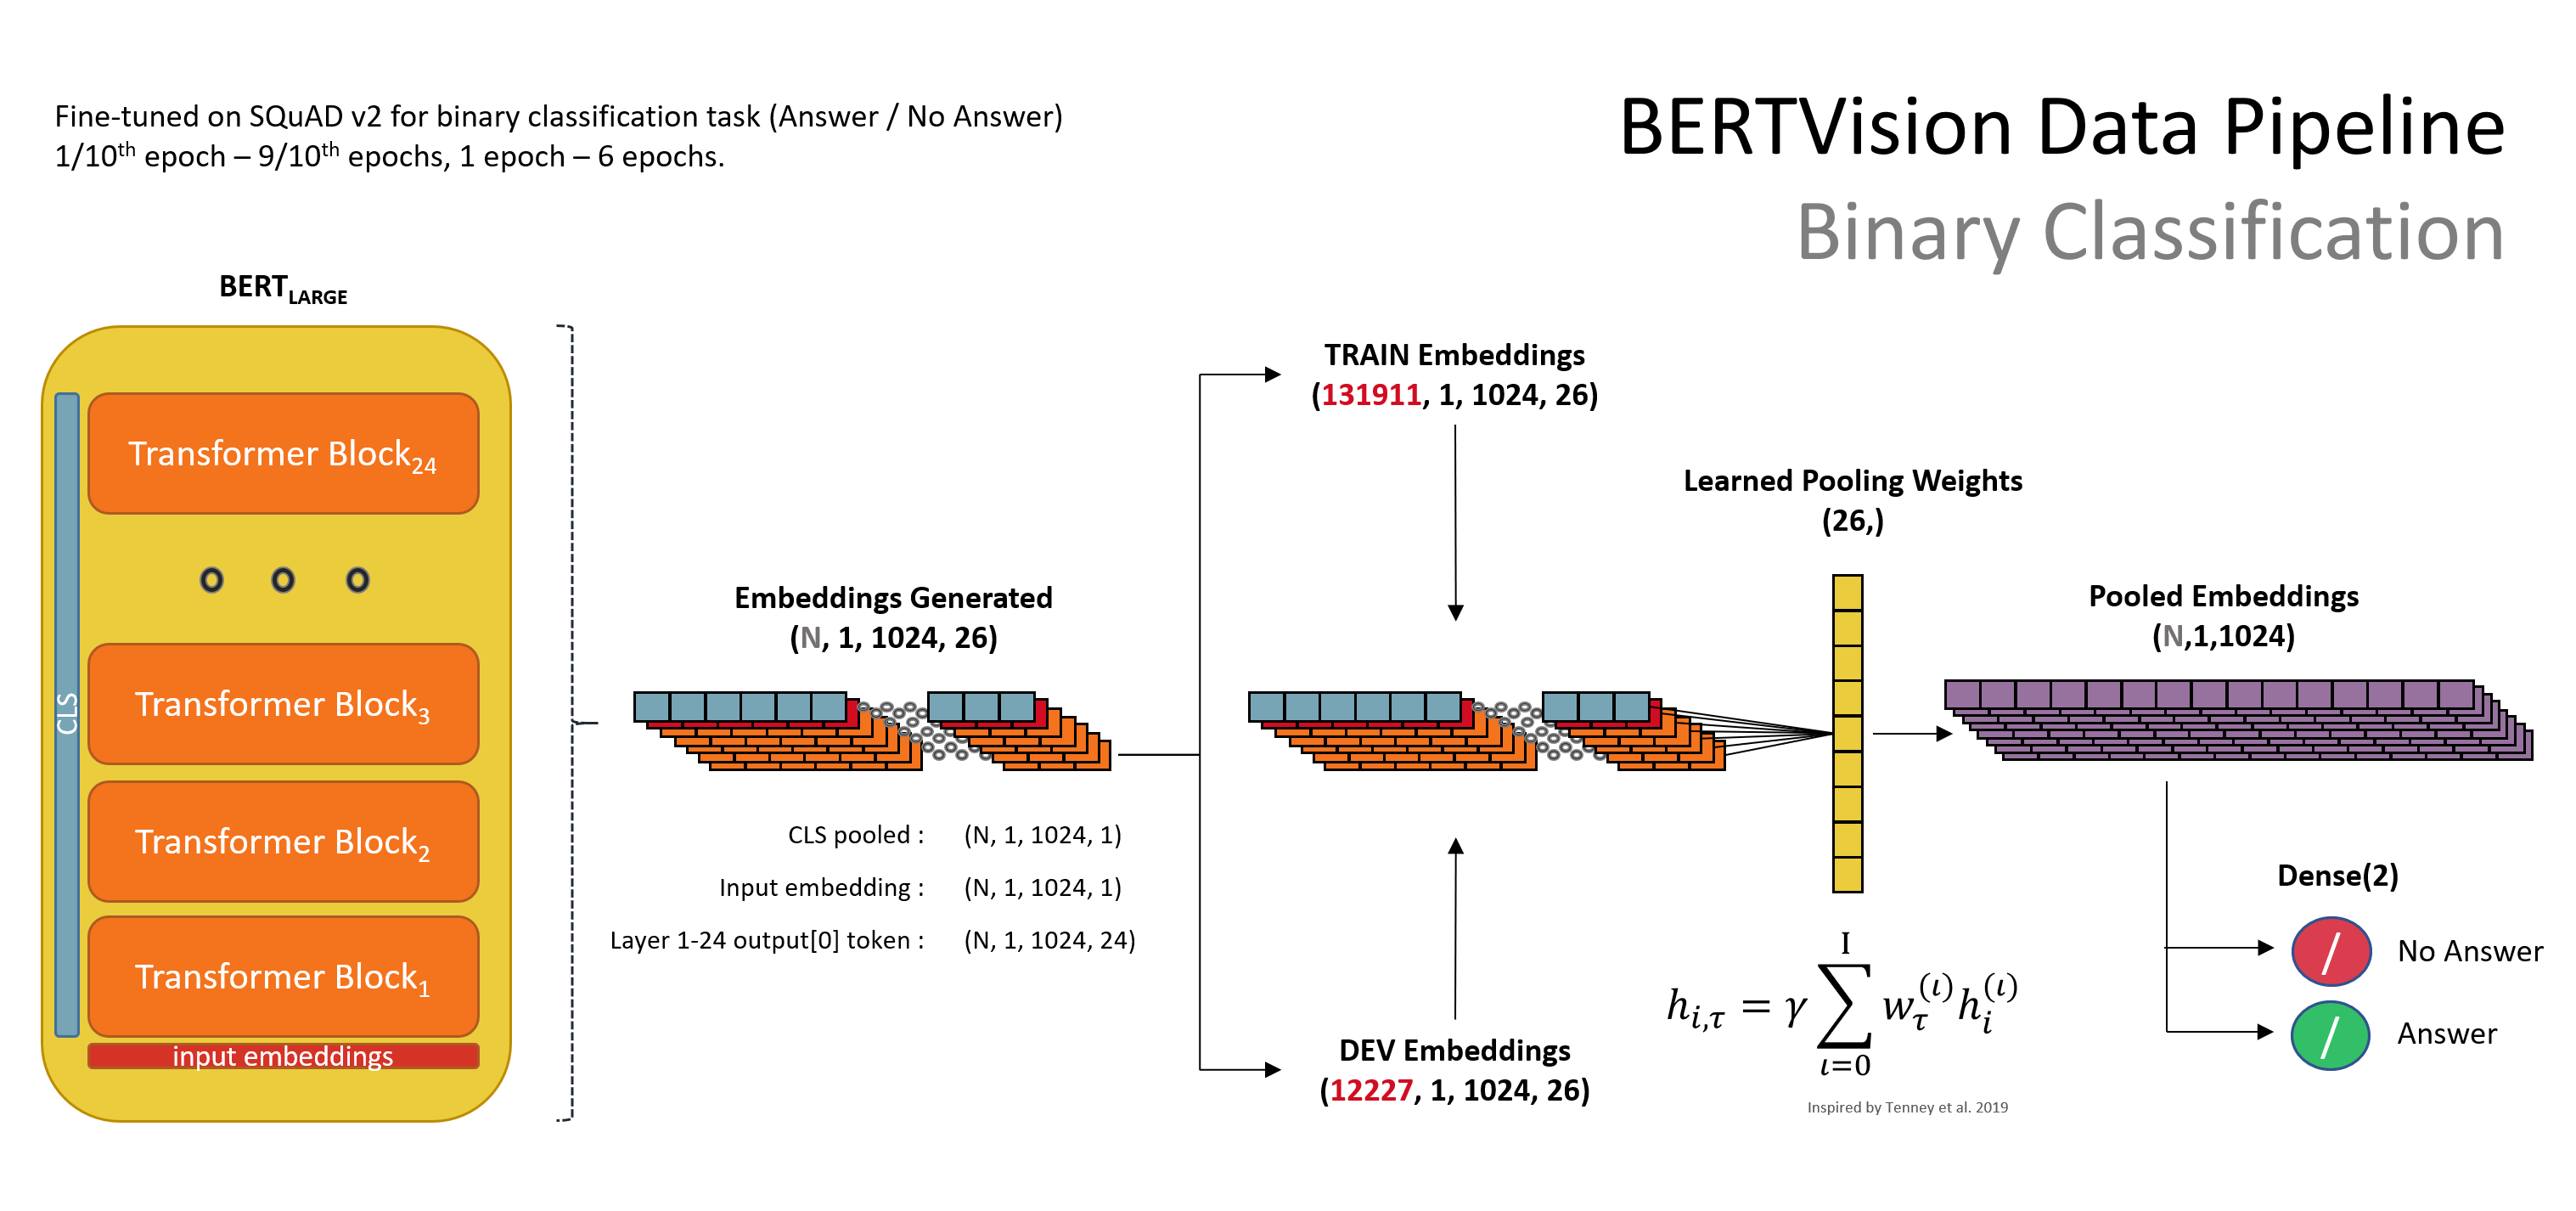
\includegraphics[width=\textwidth]{images/Data_Pipeline_Binary_Classification.png}%
	\caption{BERTVision classification data pipeline}
	\label{apdx:bertvision_classification_data_pipeline_graph}
\end{figure*}

\newpage

\subsection{Non-uniform weights}
\label{apdx:non-uniform}

Learned weights for learning pooling using the approach described in \cite{tenney-etal-2019-bert}. The model favors using later layers especially after layer 17. This is consistent with the observation in \cite{van_Aken_2019} that the last layers of BERT-base are much more accurate at supporting fact identification (which is the author’s proxy for span identification).



%----------------------------------------------------------------------------------------

\end{document}